\documentclass[11pt]{article}
\usepackage[margin=1in]{geometry}
\usepackage{graphicx}
\usepackage{booktabs}
\usepackage{array}
\usepackage{xcolor}
\usepackage{amssymb}
\usepackage[colorlinks=true,linkcolor=blue,urlcolor=blue]{hyperref}
\usepackage{titlesec}
\titlespacing*{\section}{0pt}{1.3ex}{0.6ex}
\titlespacing*{\subsection}{0pt}{1.0ex}{0.4ex}
\newcommand{\fixed}{\textcolor{green!55!black}{\textbf{Fixed}}}
\newcommand{\partialx}{\textcolor{orange!85!black}{\textbf{Partial}}}
\newcommand{\notfixed}{\textcolor{red!75!black}{\textbf{Not fixed}}}
\newcommand{\removed}{\textcolor{blue!70!black}{\textbf{Removed}}}
\setlength{\parskip}{0.4em}
\setlength{\parindent}{0pt}

\title{\vspace{-3.5em}\textbf{BabyLM: what the 2025 scores looked like, and which\\
evaluation bugs the 2026 pipeline fixed}}
\author{Working note --- \texttt{explorations/babylm2025}}
\date{\today}

\begin{document}
\maketitle
\vspace{-2.2em}

\begin{abstract}
\noindent This note does two things for a prospective 2026 BabyLM entrant. First,
it audits — against the actual code of the 2026 evaluation pipeline
(\texttt{github.com/babylm-org/babylm-eval}) — which of the concrete evaluation
bugs reported in the 2025 challenge papers were fixed. Second, it shows what the
spread of \textbf{BLiMP} and \textbf{(Super)GLUE} scores across 2025 systems
actually looks like, so that a new score can be placed in context. The short story
on the bugs: the BLiMP tie/NaN inflation and the age-of-acquisition mis-fit are
fixed, the buggy WUG morphology tasks were deleted outright, but the EWoK
``concepts-absent-from-training'' problem is a data issue that remains. The short
story on the scores: BLiMP spreads widely ($\approx$49--80) and is the metric that
actually separates systems; (Super)GLUE is compressed ($\approx$53--72) and barely
distinguishes a $10\times$ difference in training data.
\end{abstract}

\section{Sources and scope}
The evaluation bugs are those documented in the 2025 BabyLM proceedings
(\texttt{2025.babylm-main}; all 41 papers were read --- see the companion
\texttt{evidence.md}). The fix status is established by reading the 2026 pipeline
source and its git history, not from any changelog (there is none). Paper
references use the anthology number, e.g.\ (main.16). The score data are compiled
from the primary submission papers; the caveats on that are stated in
Section~\ref{sec:spread}.

\section{Which evaluation bugs were fixed in 2026?}
Table~\ref{tab:bugs} is the summary; the notes below give the mechanism and the
code evidence.

\begin{table}[h]
\centering
\small
\renewcommand{\arraystretch}{1.25}
\begin{tabular}{@{}p{3.5cm} p{5.0cm} p{4.4cm} c@{}}
\toprule
\textbf{Issue (reported by)} & \textbf{2025 behaviour} & \textbf{2026 state} & \textbf{Verdict}\\
\midrule
BLiMP tie / NaN inflation \newline (main.16) &
\texttt{torch.max} picks first index on ties; NaNs propagate; a degenerate model can report 100.0 &
NaN$\to-\infty$ and \emph{random} tie-breaking; degenerate models now score at chance (commit \texttt{9bcf1f2}, Apr 2026) &
\fixed \\

\quad --- underlying permutation items &
22 of 67 BLiMP paradigms are word-order permutations &
Same 67 paradigms still shipped; only the \emph{scoring} changed &
\partialx \\

Age-of-Acquisition mis-fit \newline (main.29) &
Unbounded sigmoid fit (\texttt{maxfev=1000}) diverges and drops most words, so the correlation uses only 1--5 points &
Bounded fit, \texttt{maxfev=20000}, per-checkpoint averaging, corrected chance ceiling, $p$-value gate (commit \texttt{7d0a6c8}, Jul 2026) &
\fixed \\

WUG evaluation bug \newline (main.14); WUG${=}100$ under morpheme tokenizers (main.21) &
Buggy morphological WUG (past/adj) correlation tasks &
Both WUG tasks \emph{deleted} from the 2026 suite (commit \texttt{9bcf1f2}) &
\removed \\

EWoK at chance: ${\sim}13\%$ of items use concepts absent from training (main.15) &
Filter only drops out-of-vocab items; no training-coverage check &
\texttt{ewok/dl\_and\_filter.py} and \texttt{vocab.txt} byte-identical; pair construction/collation fixed but coverage untouched &
\notfixed \\

Reading-time task (fragility noted by main.17, main.31) &
Surprisal--RT regression &
Unchanged except a tokenizer-loading fallback &
--- \\
\bottomrule
\end{tabular}
\caption{Status in the 2026 pipeline of evaluation bugs reported in the 2025
challenge papers. ``Verdict'' colours: \fixed{} / \partialx{} / \removed{} /
\notfixed.}
\label{tab:bugs}
\end{table}

\textbf{BLiMP tie/NaN (fixed).} In 2025, \texttt{rank\_and\_evaluate} chose the
argmax candidate with \texttt{torch.max(...)[1]}, which returns the
\emph{first} index on ties and lets NaNs create spurious maxima; an order-invariant
or degenerate model could therefore be scored as correct, and a dummy model could
report 100.0. The 2026 code first maps NaN to $-\infty$ and then breaks ties
\emph{randomly}, so a model that cannot distinguish the minimal pair now scores at
chance. This removes the inflation. It does \emph{not} remove the 22 paradigms
whose two sentences are permutations of one another --- they are still in the data
snapshot; they simply no longer inflate a degenerate model.

\textbf{Age-of-Acquisition (fixed).} The 2025 model-side sigmoid fit was unbounded
and capped at \texttt{maxfev=1000}; on many clean learning curves the shape
parameter diverged and the word was discarded, leaving the human--model correlation
computed over a handful of survivors --- exactly the ``unpassed condition on the
parameters of the fitted sigmoid'' that main.29 diagnosed. The 2026 fit is
\emph{bounded}, uses $20\times$ more evaluations, averages surprisals within each
checkpoint, corrects the chance-surprisal ceiling, and gates on a $p$-value. One
caveat: the 2026 strict \textsc{readme} reports AoA as an MSE-like quantity
computed server-side, so the exact headline number may differ from the repository's
Pearson-correlation code; only the repo-side fit could be verified here.

\textbf{WUG (removed).} Rather than repair the morphological WUG past/adj tasks,
2026 deletes them: the \texttt{rank\_and\_evaluate\_wug} routine, the task
dispatch, and the collation entries are all gone. The ``WUG${=}100.00$ under a
morpheme tokenizer'' artifact and the sign-flipping negative correlations are
therefore moot --- but so is any WUG signal.

\textbf{EWoK (not fixed).} main.15 showed EWoK sits at chance partly because
${\sim}13\%$ of its test items involve concepts that never appear in the training
corpus. That is a property of the \emph{data}, and the 2026 filter and vocabulary
files are byte-for-byte identical to 2025. Recent 2026 commits fixed how EWoK pairs
are \emph{constructed and scored} (two context-based minimal pairs; a
prediction/target matching fix), which improves correctness, but the
coverage problem --- the reason EWoK barely rises above $0.50$ --- is untouched.
Treat EWoK the same way in 2026 as in 2025: near-uninformative at this scale.

\subsection{Other changes worth knowing}
\textbf{Task list.} The 2026 strict zero-shot suite keeps BLiMP, BLiMP-Supplement,
EWoK, Entity Tracking, COMPS, reading-time and AoA, \emph{drops} both WUG tasks, and
\emph{adds} GlobalPIQA (length-normalised). Fine-tuning keeps the same seven
(Super)GLUE tasks (BoolQ, MNLI, MRPC, MultiRC, QQP, RTE, WSC; MNLI/QQP subsampled to
10k). A new \textbf{Multilingual} track (English/Dutch/Chinese) adds MultiBLiMP,
Hanzi structure/pinyin minimal pairs, and MECO reading-time.

\textbf{Aggregation.} Neither the 2025 nor the 2026 repository computes the headline
Macro Average; it is calculated server-side on the leaderboard. In 2025 it was the
mean of the accuracy (``NLP'') average and the correlation (``human-likeness'')
average --- a 50/50 split. Whether 2026 keeps that exact weighting cannot be
determined from the pipeline code, but the \emph{composition} of the two halves has
changed: the human-likeness side lost the WUG tasks, and the accuracy side gained
GlobalPIQA.

\section{What the BLiMP and (Super)GLUE spread looks like}
\label{sec:spread}

\begin{figure}[h]
\centering
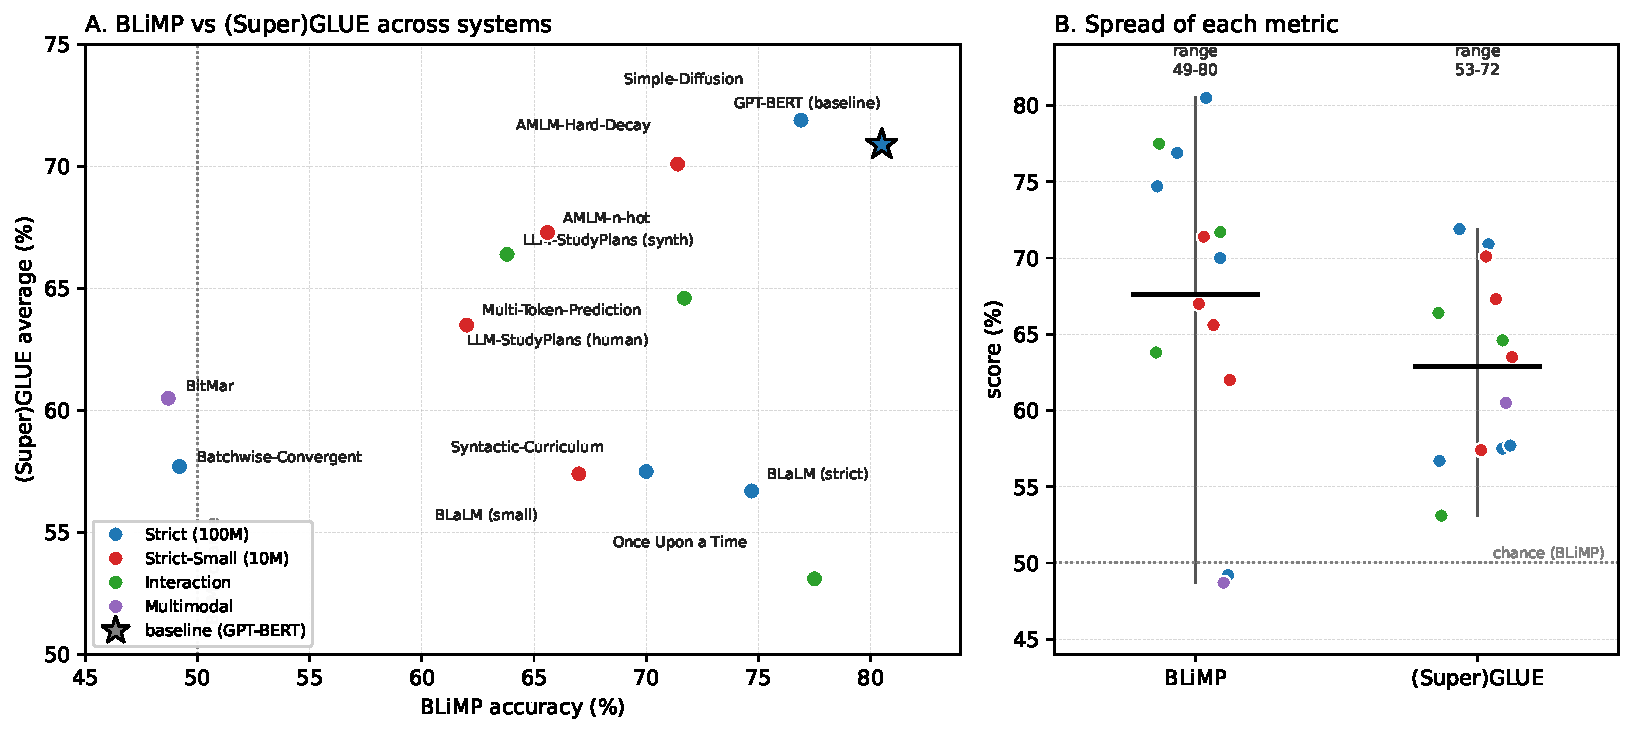
\includegraphics[width=\textwidth]{../figure/blimp_glue_spread.pdf}
\caption{BLiMP versus (Super)GLUE for a cross-section of 2025 systems.
\textbf{(A)} Each point is one system; colour is the track; the star is the
official GPT-BERT baseline. \textbf{(B)} The same values shown as a one-dimensional
spread per metric (black bar = mean, whisker = min--max). BLiMP ranges $\approx$49--80;
(Super)GLUE is compressed into $\approx$53--72. Across systems the two are only
weakly related (Pearson $r\approx0.25$). Data compiled from the primary submission
papers; each point's BLiMP and GLUE come from the \emph{same} source, but values are
as-reported (including author re-implementations of the baselines) and GLUE-vs-SuperGLUE
averaging conventions vary slightly. This is not the official leaderboard table,
which is gated.}
\label{fig:spread}
\end{figure}

Three things stand out, and they are what matter for judging a new score.

\textbf{BLiMP is the metric that separates systems.} Its range across these systems
is about 31 points (49 to 80), with a standard deviation near 9.5. A one-point BLiMP
difference low down is meaningful; near the top it is not, because the strongest
models approach the human/large-LM reference and the metric saturates.

\textbf{(Super)GLUE is compressed and scale-insensitive.} Its range is about 19
points (53 to 72), standard deviation near 6. The organisers' own finding reinforces
this: only two of seven Strict (100M-word) systems beat the best Strict-Small
(10M-word) system on GLUE. A metric that barely reflects a $10\times$ data difference
cannot finely rank models that differ by far less --- so read GLUE as a coarse band,
not a ranking.

\textbf{The two are weakly correlated, so ``good'' is metric-specific.} Systems with
strong BLiMP and mediocre GLUE (Once Upon a Time: 77.5 / 53) and the reverse
(Batchwise-Convergent: 49 / 58) both exist. A single system can look strong on one
axis and ordinary on the other; the baseline (GPT-BERT) is the rare point that is at
the top of both.

\subsection{Reference bands for placing your own score}
From Figure~\ref{fig:spread} and the challenge results, the following anchors let a
new score be judged without the leaderboard. They are approximate and track-dependent.

\begin{table}[h]
\centering
\small
\renewcommand{\arraystretch}{1.2}
\begin{tabular}{@{}l l l l l@{}}
\toprule
\textbf{Metric} & \textbf{Chance / floor} & \textbf{Weak} & \textbf{Competitive} & \textbf{Strong / reference}\\
\midrule
BLiMP        & 50 (minimal pairs)   & 50--62 & 67--75 & 76--80 (GPT-BERT); 85--89 skyline\\
(Super)GLUE  & $\approx$50 (majority)& 53--57 & 58--66 & 67--72 (GPT-BERT $\approx$71)\\
EWoK         & 50                   & \multicolumn{3}{l}{$\approx$50--54 for \emph{everyone} --- do not read differences}\\
Entity Track.& $\approx$20          & \multicolumn{3}{l}{high-variance (seed SD 6--9 pts); use only as a seeded probe}\\
\bottomrule
\end{tabular}
\caption{Rough reference bands for the metrics that carry signal, from the 2025
cross-section. ``Skyline'' for BLiMP is the human / large-LM reference reported by
the organisers.}
\label{tab:bands}
\end{table}

Practical reading: to know whether a submission is good, compare its \textbf{BLiMP}
against the GPT-BERT baseline for its track (about 80 for Strict, high-60s to low-70s
for Strict-Small) --- that is the number that most cleanly says ``ahead of'' or
``behind'' the field --- and treat \textbf{GLUE} as a wide competitive band around
the high-50s to low-70s rather than a fine ranking. Do not use EWoK or the
human-likeness tasks to decide whether a model is good; as the audit shows and the
2025 papers repeatedly found, small movements there are noise (and, for AoA in 2025,
were partly a bug now fixed).

\section{Bottom line}
The 2026 pipeline is genuinely cleaner: the two most damaging scoring bugs (BLiMP
tie/NaN inflation, AoA mis-fit) are fixed, and the unreliable WUG tasks are gone. The
one substantive issue that survives is EWoK's data-coverage problem, so EWoK remains
near-uninformative. For contextualising a score, BLiMP is the axis to trust and to
compare against the track baseline; (Super)GLUE is a coarse, compressed band; and the
rest should be read with the scepticism the 2025 submissions themselves recommended.

\end{document}
